\documentclass[12pt]{article}

% -----------------------------
% Sprache, Encoding & Fonts
% -----------------------------
\usepackage[utf8]{inputenc}
\usepackage[T1]{fontenc}
\usepackage[ngerman]{babel}
\usepackage{csquotes}     % \enquote
\usepackage{microtype}    % bessere Laufweite/Umbruch
\usepackage{ebgaramond}

% -----------------------------
% Layout & Grundpakete
% -----------------------------
\usepackage{geometry}
\geometry{margin=1in}
\usepackage{setspace}
\usepackage{parskip}

% -----------------------------
% Mathematik & Symbole
% -----------------------------
\usepackage{amsmath,amssymb,amsthm}
\usepackage{mathrsfs}

% -----------------------------
% Grafiken & Plots
% -----------------------------
\usepackage{graphicx}
\graphicspath{{./resources/images/}}
\usepackage{caption}
\usepackage{subcaption}
\usepackage{float}
\usepackage{pgfplots}
\pgfplotsset{compat=1.18}
\usepackage{tikz}
\usetikzlibrary{calc,intersections,decorations.pathreplacing,patterns,angles,quotes,shapes,arrows,positioning,automata}
\usepgfplotslibrary{fillbetween}
\usepackage[output=png]{plantuml} % <— PlantUML für UML-Diagramme

% -----------------------------
% Sonstige Nützliches
% -----------------------------
\usepackage{enumitem}
\usepackage{booktabs}
\usepackage{multicol}
\usepackage{multirow}
\usepackage{polynom}
\usepackage{tikz-cd}
\usepackage{comment}
\usepackage{fancyvrb}
\usepackage{fancyhdr}
\usepackage{etoolbox}
\usepackage{listings}
\usepackage{tkz-euclide}
\usepackage{hyperref}
\usepackage{siunitx}   % für circuitikz/Si-Einheiten
\usepackage{circuitikz}
\usepackage{bookmark}
\usepackage{tabularx}
\usepackage{ragged2e}  % für RaggedRight in Tabellenspalten

% -----------------------------
% Tabellen: neue Spaltenart (ragged) für bessere Umbrüche
% -----------------------------
\newcolumntype{Y}{>{\RaggedRight\arraybackslash}X}

% -----------------------------
% Header/Footer
% -----------------------------
\pagestyle{fancy}
\fancyhead[l]{Gruppe 12}
\fancyhead[c]{SWT \#4}
\fancyhead[r]{\today}
\fancyfoot[c]{\thepage}
\renewcommand{\headrulewidth}{0.2pt}
\setlength{\headheight}{15pt}

% Etwas mehr Flexibilität beim Zeilenumbruch
\emergencystretch=1.5em


\graphicspath{{./resources/images_4/}}

\begin{document}

\section*{A1 Test Driven Development}

Testfälle für das Steuerungssystem einer Lampe.

\begin{itemize}

    \item \textbf{T1: Ein- und Ausschalten:}  
    Die Lampe soll auf Befehl ein- und ausgeschaltet werden können.

    \item \textbf{T2: Counter-Mock:}  
    Verwende ein Mock-Objekt für die Uhr, das so konfiguriert werden kann, 
    dass Stunden als Sekunden simuliert werden. Bereite anschließend eine Reihe 
    von Operationen vor, die zu bestimmten Zeitpunkten ausgeführt werden sollen 
    (z.\,B. einfache Additionen). Überprüfe, ob die korrekte Anzahl von Operationen 
    ausgeführt wurde.

    \item \textbf{T3: Synchronisation:}  
    Überprüfe, ob sich das \texttt{TimeTracking}-Objekt korrekt mit der Systemuhr 
    des Rechners synchronisiert.

    \item \textbf{T4: Test mit Mock-Objekt:}  
    Simuliere den Fall, in dem die Lampe mit dem Mock-Objekt gesteuert wird.

    \item \textbf{T5: Test mit TimeTracking-Objekt:}  
    Teste die Lampe im realen Anwendungsfall mit dem \texttt{TimeTracking}-Objekt.

\end{itemize}

\section*{A2 Scrum}

\subsection*{[a] Vorgehen in zwei Situationen während des Sprints}

\paragraph{Fall 1: Sprintziel und alle User Stories sind \emph{vorzeitig} erfüllbar.}

\begin{enumerate}

  \item \textbf{Sprint nicht verlängern oder verkürzen} (Timeboxing beibehalten): Die Sprintdauer ist fix und wird nicht angepasst; nur Ereignisse dürfen enden, sobald ihr Zweck erfüllt ist.
  
  \item \textbf{Mit dem Product Owner (PO) \emph{Scope neu vereinbaren}:} Das Dev-Team kann, falls sinnvoll, weitere gut vorbereitete Product-Backlog-Einträge (DoR erfüllt) in den Sprint \emph{ziehen}, sofern das Sprintziel nicht gefährdet wird. Inhalt und Umfang des Sprints dürfen mit dem PO neu vereinbart werden.

  \item \textbf{Weitere Inkremente liefern:} Mehrere Inkremente pro Sprint sind möglich; vorzeitige Lieferung ist erlaubt, solange die \emph{Definition of Done} eingehalten wird.
  
  \item \textbf{Qualität stärken \& Schulden abbauen:} Falls keine zusätzlichen, wertvollen Stories verfügbar sind: Refactoring, Testausbau und Dokumentation gemäß DoD priorisieren.

  \item \textbf{Sprintabbruch nur in Ausnahmefällen:} Wird das Sprintziel obsolet, kann ausschließlich der PO den Sprint abbrechen.

\end{enumerate}

\paragraph{Fall 2: Sprintziel und User Stories sind \emph{sehr wahrscheinlich} nicht rechtzeitig erfüllbar.}

\begin{enumerate}

  \item \textbf{Transparenz \& Re-Planung im Daily Scrum:} Fortschritt und Hindernisse offenlegen; Plan anpassen, um das Sprintziel bestmöglich zu erreichen.
  
  \item \textbf{Scope mit dem PO neu verhandeln:} Umfang des Sprint Backlogs \emph{reduzieren} (z.\,B.\ niedere Prioritäten verschieben), ohne das Sprintziel oder Qualitätsansprüche zu gefährden. \emph{Qualität nimmt nicht ab}.

  \item \textbf{Impediments beseitigen lassen:} Der Scrum Master unterstützt aktiv beim Entfernen von Hindernissen.
  
  \item \textbf{DoD nicht aufweichen:} Keine Abstriche bei Qualitätskriterien; unvollständige Arbeit bleibt \enquote{nicht fertig} und wird transparent gemacht.
  
  \item \textbf{Keine Sprintverlängerung und kein \enquote{Personen nachschieben}:} Die Sprintlänge bleibt fix; zusätzliches Personal macht späte Projekte oft noch später (Brooks’sches Gesetz).
  
  \item \textbf{Stakeholder-Einbindung:} Ergebnisse und Anpassungsbedarf spätestens im Sprint Review demonstrieren und besprechen.

\end{enumerate}

\newpage

\subsection*{[b] Sehr kurze (z.\,B.\ 1 Woche) vs.\ sehr lange (z.\,B.\ 8 Wochen) Sprintlängen}

\begin{table}[h]
\centering
\renewcommand{\arraystretch}{1.15}
\begin{tabularx}{\textwidth}{@{} l Y Y @{}}
\toprule
& \textbf{Vorteile} & \textbf{Nachteile} \\
\midrule
\textbf{Kurz (\(\approx\) 1 Woche)} &
\begin{itemize}[leftmargin=*]
  \item Sehr häufiges Feedback; schnelle Kurskorrekturen.
  \item Frühe Risikosichtbarkeit und kurze Lernschleifen.
  \item Hohe Fokusdisziplin auf kleine, klar geschnittene Inkremente.
  \item Regelmäßige Lieferbarkeit und verlässlicher Takt.
\end{itemize}
&
\begin{itemize}[leftmargin=*]
  \item Relativ hoher Event-Overhead (Planning/Review/Retrospektive) im Verhältnis zur Umsetzung.
  \item Gefahr von zu kleinteiligen Stories bzw.\ Stückelung.
  \item Mehr Planungsdruck; häufigere Schätz-/Refinement-Zyklen.
\end{itemize}
\\
\midrule
\textbf{Lang (\(\approx\) 8 Wochen)} &
\begin{itemize}[leftmargin=*]
  \item Weniger \enquote{Ceremony}-Overhead pro Arbeitswoche.
  \item Mehr Zeit für komplexe Features innerhalb eines Sprints.
  \item Weniger Kontextwechsel durch selteneres Planen/Reviewen.
\end{itemize}
&
\begin{itemize}[leftmargin=*]
  \item Weniger Feedback; Risiken werden später sichtbar.
  \item Größere Batches/WIP $\rightarrow$ spätere Integration, höhere Fehlerrisiken.
  \item Geringere Agilität; Scope Creep wird später erkannt.
\end{itemize}
\\
\bottomrule
\end{tabularx}
\caption{Vier-Felder-Tafel: kurze vs.\ lange Sprintlängen.}
\end{table}

\section*{A3 Smart Phone State UML}
 
\begin{plantuml}
@startuml
title UML-Zustandsdiagramm: Smartphone-Steuerung

[*] --> Ausgeschaltet : Start

state Ausgeschaltet

state Normal 

state Energiesparen

state Standby

Ausgeschaltet -down-> Normal : AnAus_Taste_drücken

Normal -up-> Ausgeschaltet : AnAus_Taste_drücken

Normal -down-> Energiesparen : [nach 15s Inaktivität]

Energiesparen -up-> Normal : Home_Taste_drücken

Energiesparen -down-> Standby : [nach 60s]

Standby -up-> Energiesparen : Home_Taste_drücken

Normal -left-> Normal : Home_Taste_drücken\noder Bildschirmgeste

Ausgeschaltet -right-> [*] : Ende

@enduml
  
\end{plantuml}


\begin{figure}[H]
    \centering
    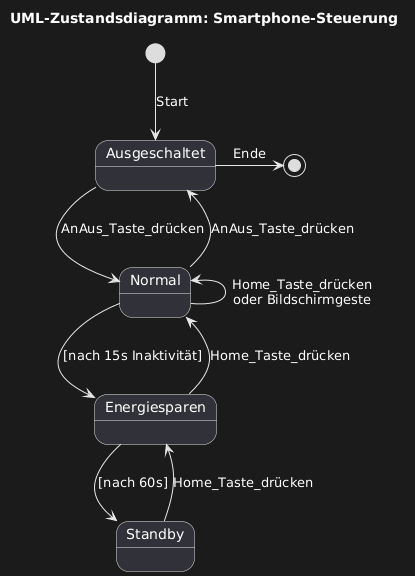
\includegraphics[width=\linewidth, height=0.6\textheight,keepaspectratio]{resources/images_4/3.png}
  \end{figure}


\section*{Aufgabe 4 - UML-Klassendiagramm/Zustandsdiagramm: Stapelspeicher}

\subsection*{Klassendiagramm (\enquote{Stack<TElement>})}
% Eindeutiger Ausgabename für das folgende Diagramm
\def\PlantUMLJobname{SWT-class}
\begin{plantuml}
@startuml
hide empty members
skinparam classAttributeIconSize 0

' Parametrisierte Klasse mit Template-Parameter TElement
class Stack<TElement> <<template>> {
  - capacity : Integer {readOnly}
  - count    : Integer {readOnly}

  + Stack(capacity : Integer)
  + push(e : TElement) : void
  + pop()  : TElement [0..1]
  + peek() : TElement [0..1]
}

' Invarianten und Randbedingungen nach Aufgabenstellung / Folien
note right of Stack
  {invariant: capacity >= 2}
  {constraint: TElement ist ein Referenztyp (kein primitiver Typ)}
end note
@enduml
\end{plantuml}

\subsection*{Zustandsdiagramm (Call Events, Guards, Effects)}
% Eindeutiger Ausgabename für das folgende Diagramm
\def\PlantUMLJobname{SWT-states}
\begin{plantuml}
@startuml
hide empty description

[*] --> Empty

state "Empty" as Empty
state "Filled" as Filled
state "Full" as Full

' --- Empty ---
Empty --> Filled : push(e:TElement)\n[count < capacity]\n/ count := count + 1
Empty --> Empty  : pop()\n[count == 0]\n/ return null
Empty --> Empty  : peek()\n[count == 0]\n/ return null

' --- Filled ---
Filled --> Full   : push(e:TElement)\n[count + 1 == capacity]\n/ count := count + 1
Filled --> Filled : push(e:TElement)\n[count + 1 <  capacity]\n/ count := count + 1
Filled --> Empty  : pop()\n[count - 1 == 0]\n/ count := count - 1
Filled --> Filled : pop()\n[count - 1  > 0]\n/ count := count - 1
Filled --> Filled : peek()\n[count > 0]\n/ return top

' --- Full ---
Full --> Full   : push(e:TElement)\n[count == capacity]\n/ no-op
Full --> Empty  : pop()\n[count - 1 == 0]\n/ count := count - 1
Full --> Filled : pop()\n[count - 1  > 0]\n/ count := count - 1
Full --> Full   : peek()\n[count > 0]\n/ return top

' Ende im Zustand Empty
Empty --> [*] : dispose()
@enduml
\end{plantuml}

\end{document}
